% MICCAI 2027 submission draft, LNCS format. Built from paper/miccai/DRAFT.md.
% Anonymized for double-blind review.
\documentclass[runningheads]{llncs}
\usepackage[T1]{fontenc}
\usepackage{graphicx}
\usepackage{booktabs}
\usepackage{amsmath}
\usepackage{url}
\usepackage[hidelinks]{hyperref}

\begin{document}

\title{When Tooth-Numbering Detectors Fail Together: A Position-Only Baseline and Closed Gaps on Panoramic X-rays}
\titlerunning{When Tooth-Numbering Detectors Fail Together}
\author{Anonymized Authors}
\authorrunning{Anonymized Authors}
\institute{Anonymized Affiliations}

\maketitle

\begin{abstract}
Tooth-numbering models for panoramic X-rays report high accuracy, but the
X-ray format places each tooth in a predictable spot, so part of that
accuracy could come from position rather than appearance. We measure this
with a position-only baseline: a classifier that sees each tooth's bounding
box and no pixels. On 425 uncropped panoramic X-rays (11,602 teeth) with
five-fold cross-validation grouped by X-ray, it numbers 78.5\% of teeth
correctly. Three detectors of different design (YOLOv8x, RT-DETR-l, Faster
R-CNN) beat it by 14.3 to 16.7 percentage points, on all 32 tooth numbers,
and the gap replicates on two further splits. Their errors still follow
position. On 1.4\% of teeth all three detectors give the same wrong number,
and in 91\% of these the position-only model gives it too, against under 7\%
by chance. A sequence of interventions locates these shared errors.
Shifting the whole image barely changes the detectors' answers, and masking
distant context rarely fixes them. They sit next to a missing tooth five
times as often as correct teeth and usually take the missing tooth's
number, and they occur where the neighbors have closed the space (AUROC
0.78). Closing a gap on purpose reproduces them: when a neighbor is moved
into an erased tooth's space, all three detectors give it the missing
number 21\% of the time, against 0.2\% when the space is left open. We release the per-tooth table and a scorer so new models can be
compared with the baseline and on the shared failures.
\keywords{Tooth numbering \and Panoramic radiography \and Shortcut learning \and Error consistency}
\end{abstract}

\section{Introduction}

Assigning each tooth its FDI number is the first step of most automated
dental charting: a caries or a periapical lesion found by a detector is
only useful once it is attached to the right tooth. Public benchmarks such
as DENTEX~\cite{hamamci2023dentex} score numbering together with detection,
and reported accuracies are high.

Panoramic X-rays are a strongly standardized format. The patient bites on a
guide, the arch runs left to right across the image, and each tooth number
has a typical location. This invites a shortcut~\cite{geirhos2020shortcut}:
a model can get many numbers right from where a box sits, without reading
the tooth. Such a shortcut would be invisible in aggregate accuracy and
would fail on the patients who differ from the typical arch, for example
after extractions.

We ask how much of tooth numbering position alone explains, and whether
detectors fail where position fails. Our contributions:
(1)~a position-only baseline, trained in seconds on six box features, that
numbers 78.5\% of teeth correctly under grouped cross-validation, with three
detectors beating it by 14 to 17 points on every tooth number;
(2)~an error analysis showing that the detectors' shared errors are
position-like;
(3)~interventions and checks (image shift, context masking, tooth
erasure, a space-closure measure and gap closure on purpose) that place
these errors at closed gaps, next to a
missing tooth whose neighbors have moved together so the arch looks
complete; and
(4)~a released per-tooth benchmark with folds, reference predictions and a
scorer.

\section{Related Work}

\textbf{Tooth numbering.} Detection-based numbering on panoramic X-rays is
standard, with DENTEX~\cite{hamamci2023dentex} and hierarchical diffusion
detectors~\cite{hamamci2023hierarchical} as recent examples and many DENTEX
challenge entries building on YOLO or DETR
variants~\cite{he2023dentex,mei2023yolortho,choi2023detdet}. Some methods
use the arch layout as an explicit prior~\cite{budagam2024oralbbnet}.
Evaluations report accuracy or mAP; we found none that compares a model with
what position alone achieves on the same teeth.

\textbf{Shortcut learning.} Models can rely on cues that correlate with the
label in training data, from skin markings in
dermoscopy~\cite{winkler2019markings} to site-specific features in chest
X-rays~\cite{degrave2021covid} and segmentation~\cite{lin2024shortcut}; see
also~\cite{hill2024shortcutting,cajas2026shortkit}. These studies show a
shortcut by removing or altering the cue. We use the same logic for a cue
that is partly legitimate: position does carry information about tooth
number.

\textbf{Error consistency.} Whether two models fail on the same inputs
beyond chance is measured by error-consistency
kappa~\cite{geirhos2020consistency}. We go one step further and compare the
wrong answers themselves.

\section{Methods}

\textbf{Data and splits.} UFBA-425~\cite{budagam2025ufba} contains 425
panoramic X-rays ($512\times512$ pixels) with per-tooth masks labeled by FDI
number (32 classes, third molars included). Each tooth's box is the full
extent of its mask, giving 11,602 teeth. We use the original X-rays only;
an augmented export of this data adds randomly cropped copies, which move
teeth in the frame and lowered position-only accuracy by about 8 points in
our earlier splits. X-rays are split into five folds stratified by the
dataset's categories; each training fold holds out 15\% of its X-rays for
model selection, and each X-ray is tested once by models that never saw it.
Two further splits (other seeds) share at most about a quarter of any test
fold with the first.

\textbf{Models.} The position-only baseline is a gradient-boosted tree
classifier (scikit-learn HistGradientBoosting, default settings) on six
features of the labeled box: center $x$ and $y$, width, height, area and
aspect ratio, relative to image size. It never sees pixels. The detectors
are YOLOv8x~\cite{jocher2023yolov8}, RT-DETR-l~\cite{zhao2024rtdetr} and
Faster R-CNN~\cite{ren2015faster} with a ResNet-50 FPN
backbone~\cite{li2021benchmarking}, all from COCO weights: a single-stage
CNN, a transformer and a two-stage CNN, from two separate code bases. Each
is trained for 30 epochs at 640 pixels with horizontal flips off (a flip
swaps left and right tooth numbers); Faster R-CNN uses SGD with a learning
rate scaled to its batch of 2. The epoch with the best validation fitness
($0.1\,\mathrm{mAP}_{50} + 0.9\,\mathrm{mAP}_{50:95}$) is kept.

\textbf{Scoring.} Detections with confidence at least 0.5 are matched
one-to-one to labeled teeth at IoU at least 0.5, highest confidence first,
regardless of class. A tooth with no match counts as wrong. Top-1 is the
share of labeled teeth matched and given the right number, which puts the
detectors and the baseline (which always answers) on the same teeth. We
also report numbered F1, which counts extra boxes. CIs are 95\% intervals
from 10,000 bootstrap draws of X-rays, paired for differences. Each
experiment's decision rule was written and frozen before it was run. A
tooth is a \emph{joint failure} when all three detectors and the
position-only model are wrong and the detectors give the same answer. The
\emph{position match} is the share of joint failures where the
position-only model also gives that answer; its chance level comes from
shuffling the position-only answers among the joint failures.

\textbf{Interventions.} \emph{Shift:} the whole image is translated by
$\pm10\%$ of its width (about two tooth widths), labels moved to match.
\emph{Context masking:} everything outside a tooth's box widened by $k$ box
widths and heights ($k=0.5,1,2$) is blacked out. \emph{Missing neighbor:} an
adjacent arch position has no labeled tooth. \emph{Tooth erasure:} for up to
three teeth per X-ray with both neighbors present, the tooth's mask (dilated
3 px) is inpainted~\cite{telea2004inpainting}, and we ask whether a
correctly numbered neighbor now takes the erased tooth's number; controls
are the teeth two places away and a sham inpaint over bone. \emph{Space
closure:} for each missing tooth with both neighbors present, $S$ is the
shortest distance between the neighbors' masks over the missing tooth's
median width (0 when they touch). \emph{Gap closure:} after erasing a
target tooth, its distal neighbor is cut out and pasted shifted toward the
gap by half or all of the distance at which its mask touches the tooth on
the other side, with its box moved to match.

\section{Results}

\begin{table}[t]
\caption{Top-1 on 11,602 teeth (split 0, 95\% CI) and the gap over the
position-only model. F1 counts extra boxes. Splits 2, 3: gap on two
further random splits.}\label{tab:main}
\centering
\setlength{\tabcolsep}{4pt}
\begin{tabular}{lcccc}
\toprule
 & Top-1 (\%) & Gap (points) & Numbered F1 & Splits 2, 3 gap \\
\midrule
Position-only & 78.5 (76.9--80.0) & & & \\
YOLOv8x & 95.0 (94.2--95.8) & 16.5 (15.1--17.9) & 95.0 & 15.8, 16.4 \\
RT-DETR-l & 95.2 (94.4--95.9) & 16.7 (15.3--18.1) & 92.3 & 15.9, 16.4 \\
Faster R-CNN & 92.8 (91.9--93.7) & 14.3 (13.0--15.7) & 89.6 & 13.8, 14.3 \\
\bottomrule
\end{tabular}
\end{table}

\textbf{Position explains most; detectors add 14 to 17 points.}
Table~\ref{tab:main}. Position alone numbers more than three in four teeth.
Each detector beats it on all 32 tooth numbers; the per-number gap is
smallest at the third molars (4.3 to 5.8 points) and largest at the lower
central incisors (up to 25.5). Given the detectors' own predicted boxes
instead of labeled ones, the baseline does slightly better (79.0 to 80.2\%)
and the gap is 14.5 to 16.2 points, so labeled boxes do not flatter it. On
two further splits every gap falls inside the first split's CI. YOLOv8x and
RT-DETR-l tie on top-1 (difference 0.17 against a minimum detectable
difference of 0.50), but RT-DETR-l leaves about 1.9 unmatched boxes per
X-ray against 0.4, which lowers its F1 by 2.7 points.

\textbf{Shared errors follow position.} 161 teeth (1.4\%) are joint
failures. In 91.3\% of them the position-only model gives the same wrong
number, against a permutation 95th percentile of 6.8\%, and 94.4\% of the
shared wrong numbers are one place away in the same quadrant. The detectors
are about as confident on these teeth as on correct ones (AUROC 0.53 to
0.66), so a confidence threshold does not find them, and neither does a
rule based on the detectors' second choices. About 10\% of joint failures
may be label errors by confident learning~\cite{northcutt2021confident};
without them the position match is 91.7\%.

\textbf{Not absolute position, not distant context.} Shifting the image by
two tooth widths, which leaves the position-only model right on under 9\% of
teeth, changes the detectors' top-1 by under 0.3 points. Masking everything
beyond one box width costs Faster R-CNN and RT-DETR-l about 26 points on
correctly numbered teeth (YOLOv8x 9.6), but among detected joint failures 74
to 93\% keep the shared wrong number.

\textbf{Next to missing teeth.} 44.7\% of joint failures have a missing
neighbor, against 8.5\% of teeth all three detectors get right (ratio 5.3,
CI 4.2 to 6.6). 67 of the 72 joint failures next to a gap (93\%) take the
missing tooth's number. Teeth that only the position-only model gets wrong
have a missing neighbor 10.5\% of the time: gaps are not where position
fails in general, but where position and the detectors fail together.

\begin{figure}[t]
\centering
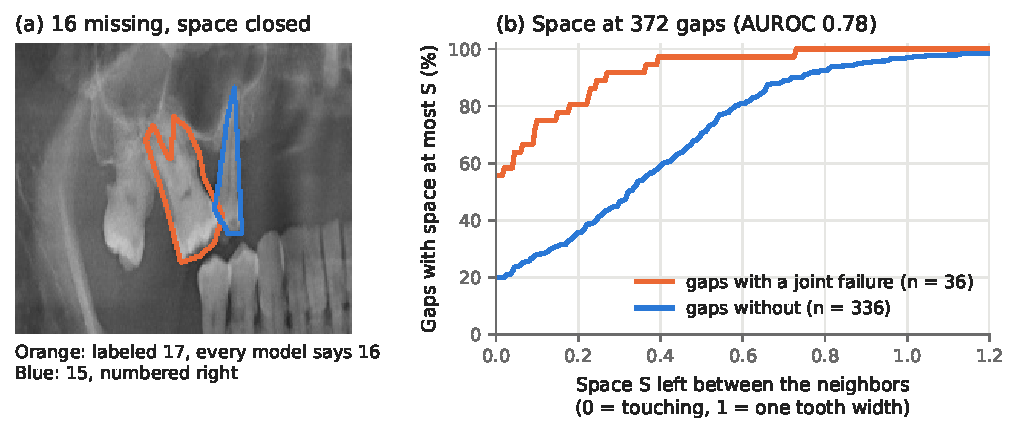
\includegraphics[width=\textwidth]{fig_closed_gap.pdf}
\caption{(a) A closed gap: tooth 16 is missing and its neighbors' outlines
touch. All three detectors and the position-only model number tooth 17 as
16. (b) Share of the 372 gaps with both neighbors present whose space is at
most $S$, for gaps with and without a joint failure.}\label{fig:gap}
\end{figure}

\textbf{At closed gaps.} Fig.~\ref{fig:gap}. Across 372 missing teeth with
both neighbors present, the space left between the neighbors separates gaps
with a joint failure from gaps without one (AUROC 0.78, CI 0.70 to 0.84;
median $S$ 0.00 against 0.32). 56\% of these errors sit at gaps whose
neighbors touch, against 20\% of other gaps. Each detector's own errors
track closure as well (AUROC 0.74 to 0.79), more than the position-only
model's (0.68).

\textbf{An open gap is not enough.} Erasing a tooth makes a correctly
numbered neighbor take its number in 2.0\% (YOLOv8x), 4.4\% (RT-DETR-l)
and 5.7\% (Faster R-CNN) of cases, against 0 to 0.2\% for both controls.
But all three detectors do it to the same neighbor in only 4 of 2,260 cases
(0.18\%).

\textbf{Closing the gap reproduces the shared error.} For the same erased
teeth, we moved the distal neighbor sideways until it touched the tooth on
the other side. Of 1,114 moved teeth that all three detectors numbered
right on the intact X-ray, all three gave the missing tooth's number to
0.18\% with the space open, 2.9\% when moved halfway and 20.8\% when moved
all the way (difference from open 20.7 points, CI 18.2 to 23.1); each
detector alone did so 38 to 42\% of the time. Models trained on two further
splits give the same result (22.5\% and 21.8\% at full closure, at most
0.1\% open). Tipping
the neighbor about its root apex until its crown touches, which is closer
to how real teeth drift, gives 9.4\% (CI 7.7 to 11.0; 9.3\% on the seed 1 models), near the 11\% per
neighbor at real closed gaps; cutting the tooth out and pasting it back
unmoved gives 0.0\%, so paste edges do not cause the effect. A moved tooth keeps its own
shape, so the detectors number it by the slot it occupies.

\section{Discussion}

The detectors read teeth: they do not number by position in the frame, and
they beat a position-only model on every tooth. Yet their rare shared
errors are the position-only model's errors, and our results show where
they happen. When a tooth is missing and its neighbors have moved together,
the arch shows no gap. Counting along it gives the tooth next to the closed
space the missing tooth's number, and that tooth also sits roughly where the
missing one would. Appearance, context and position then point the same
way, and every model follows. An inpainted gap leaves a full-width space and
does not create this agreement; closing it does.

Two practical points follow. A position-only baseline is cheap and should
be reported with tooth-numbering results: on standardized panoramic X-rays
it sets a high floor, and the margin above it is what a model contributes.
And the errors that different models share are not found by confidence; a
review rule from outside the model works better: check the numbering next
to every missing tooth, especially where the space has closed. Here such a
rule catches 97\% of the shared errors at gaps but flags many gaps without
one (precision 13\%), since most gaps are partly closed. The rule can run
on a model's own output: flagging teeth next to a position the detector
left empty, or sharing a number, marks 12 to 16\% of teeth and catches 41
to 47\% of the shared errors on every split, against 17 to 32\% for the
same number of least-confident teeth (our pre-set 1.5-fold bar was met on
two of three splits). Training does
not remove the error easily: YOLOv8x retrained with simulated missing and
closed teeth numbered teeth next to real gaps no better than a retrained
control ($+0.1$ points, CI $-1.6$ to $1.7$).

\textbf{Limitations.} One dataset from one source, a single annotation per
tooth and no demographic data; we did not validate on an external dataset
such as DENTEX. The interventions slide or tip a tooth within the image
plane only (real teeth also rotate about their long axis), and masks
on a 2D projection can touch when the teeth do not. Third-molar and longer gaps,
which hold most missing positions, are outside the closure analysis. Two
further splits, and retraining on the same split with a new seed, replicate
the main numbers; about a third of the jointly failed teeth change with
training randomness alone (overlap 0.63, against 0.54 to 0.57 across splits). About 10\% of joint failures may be label errors.

\section{Conclusion}

On uncropped panoramic X-rays, position alone numbers 78.5\% of teeth and
detectors add 14 to 17 points. The few errors they share follow position
and concentrate next to missing teeth whose neighbors have closed the
space. We release the per-tooth table and scorer so that new models can be
measured against the baseline and on these shared failures.

% Disclosure of Interests: required by Springer at camera-ready only. To be
% written by the author after acceptance.

\bibliographystyle{splncs04}
\bibliography{refs}

\end{document}
